\title{Event-Driven Architecture}
\author{Richard Thomas}
\date{\week{6}}

\maketitle

\section{Introduction}

Event-driven is an asynchronous\footnote{Asynchronous means that actions can take place in parallel.} architectural style.
It reacts to events, which is different to the common view of many systems that respond to requests.
The service-based architecture example for the Sahara eCommerce system is designed to process requests.
A customer \emph{requests} to view a product's details through a REST API and receives a response with the result.
Similarly, a customer adding a product to their shopping cart is another request.

An event could be a scenario where Sahara held auctions and customers could bid for products.
A customer would send a message to the Sahara eCommerce system initiating the \emph{event} of making a bid.
Upon receiving the bid event, the system would process the bid.
This would involve checking the bid against the current high bid and dealing with multiple customers bidding on the same item at the same time.
Each customer's bid may be for different amounts.
The system needs to determine the new high bid, and if there were concurrent bids, which is the highest bid.
The system would then notify all bidders of the new high bid.

Events provide a mechanism to manage asynchronous communication.
An event is sent to be handled, and the sender can continue with other tasks while the event is being processed.
If necessary, the handler can send a message back to the sender indicating the result of the event processing.

There are two basic approaches to implementing an event-driven architecture.
The terminology is that these are different \emph{topologies}, as they have different high-level structures.
The \emph{broker topology} is the simpler of the two and is optimised for performance, responsiveness, scalability, extensibility, and low coupling.
The \emph{mediator topology} is more complex but is designed to provide reliability, process control, and error handling.


\section{Broker Topology}

\subsection{Terminology}

The service-based architecture consists of four elements.
The \emph{user interface}, \emph{services}, \emph{service APIs}, and \emph{database}, as shown in figure \ref{fig:service-based-arch}.

\begin{description}
    \item[User Interface] provides users access to the system functionality.
    \item[Services] implement functionality for a single, independent business process.
    \item[Service APIs] provide a communication mechanism between the user interface and each service.
    \item[Database] stores the persistent data for the system.
\end{description}

The user interface runs as a standalone process to manage user interactions.
It communicates with the services through their service APIs to invoke system behaviour.
This requires a remote access communication protocol, such as REST, a message transport service,
remote method invocation, \link{SOAP}{https://www.w3schools.com/xml/xml_soap.asp} or some other protocol.

To reduce coupling between the user interface and the service APIs, and to provide easier extensibility, the user interface often uses a
\link{service locator design pattern}{https://www.baeldung.com/java-service-locator-pattern} to manage access to the services%
\footnote{Martin Fowler provides good commentary about using the service locator pattern at \url{https://martinfowler.com/articles/injection.html\#UsingAServiceLocator}.
He expands further on some tradeoffs of the pattern than other more superficial descriptions of the pattern.}.
This provides a registry of the services and the details of the API of each service.
The user interface uses the registry to retrieve an object that communicates with a service through its API.
This also makes it easier to add new services to the application, as the details of the new service are encapsulated in the registry.

Services implement the application logic for independent business processes.
These are often called ``coarse-grained'' services, as each one implements a significant part of the system's functionality.
Each service is deployed on its own computing infrastructure.
Commonly, there is a single instance of each service but it is possible to run multiple instances of services.
Multiple instances of services improves availability because if one instance goes down, other instances can handle future requests from the user interface.
To provide higher reliability, in the context of running multiple instances of a service, it should implement the
\link{stateless service pattern}{https://www.oreilly.com/library/view/design-patterns-and/9781786463593/f47b37fc-6fc9-4f0b-8cd9-2f41cb364509.xhtml}.
A system running multiple instances of a service, that does not implement the stateless service pattern,
would still have higher availability if a service instance went down, as other instances could handle future requests.
But, any user in the middle of performing a business process would need to restart their activity, thus lowering system reliability.

Services implement their own service API using the \link{façade design pattern}{https://refactoring.guru/design-patterns/facade}.
This defines the communication protocol used between the user interface and the service.
For simplicity, usually all services use the same communication protocol.
The façade design pattern reduces coupling between the user interface and the services,
as the user interface does not depend on the implementation details of the services.

The service API provides the benefit that different user interfaces can all use the same services.
For example, an application with web and mobile interfaces could use the same set of distributed domain services.

The database stores persistent data for the system.
Often, a single database is shared by all the services as it is common that some data will be shared between services.
A shared database makes it easier to maintain data integrity and consistency.
This is because each service implements a single business process
and can usually perform all transaction management related to the data involved in the process.
For example, the ProductPurchasing service for an on-line store can manage the entire database transaction for making an order.
If the product is no longer available or payment fails, the service can rollback the transaction to ensure data integrity.


\section{Design Considerations}\label{sec:design-considerations}

A service-based architecture is typically used for medium-sized systems.
This is because the user interface interacts with all services through their APIs.
The user interface becomes more complicated when it has to deal with many services.
If the services follow the common approach of using a shared database,
it means the the greater the number of services, the more complicated the database design becomes.
There is also a potential performance bottleneck if many services are using a shared database.
Strategies to improve database performance, like replicated databases, defeat some of the benefits of a shared database (e.g. consistency).
Typically a service-based architecture will have six to twelve domain services.
There is no specific upper or lower limit on the number of services allowed,
it is a tradeoff that architects make based on all the requirements for the system.

Coarsed-grained services will usually have some internal complexity that requires some architectural structure.
This internal structure may follow either technical or domain partitioning.
Technical partitioning will typically consist of three layers, the API façade, business logic and persistence.
Domain partitioning will break the service domain into smaller components related to each part of the domain's behaviour.
For example, the ProductPurchasing service domain may have components for the internal behaviours of checking out,
payment and inventory adjustment. Payment would use an API to process payment through a financial service gateway.
Figure \ref{fig:service-partitions} provides an example of the structure for both technical and domain partitioning of a service.

%\begin{figure}[h!]
%    \centering
%    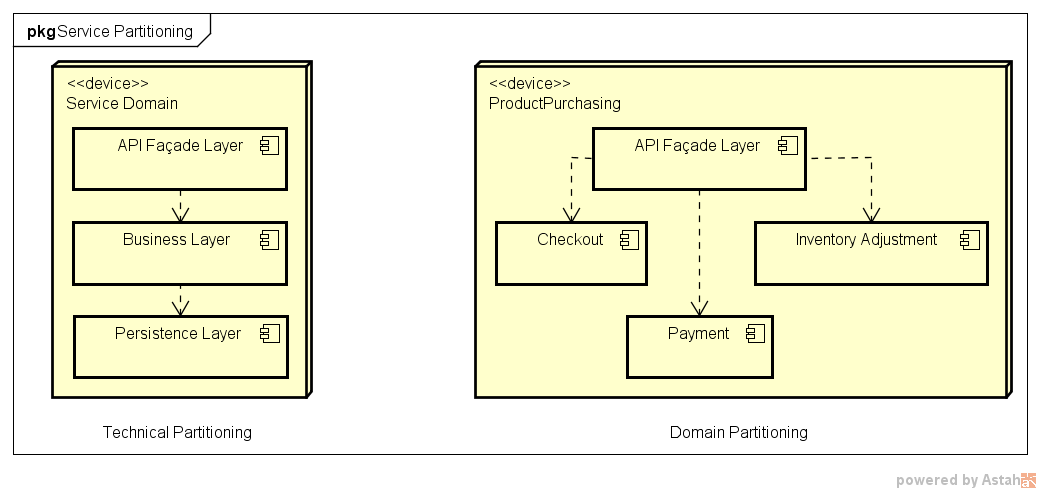
\includegraphics[trim=38 38 19 45,clip,width=\textwidth]{diagrams/service-partitions.png}
%    \vspace{-10pt}
%    \caption{Partitioning options for a service domain.}
%    \label{fig:service-partitions}
%\end{figure}

Consequences of a shared database are increased data coupling between the services and lower testability.
Increased data coupling means that if one service changes its persistent data,
then all services that share that data need to be updated, as well as the tables storing the data in the database.
Lower testability is the consequence of shared data and services implementing complete business processes.
A small change to one part of the service requires the entire service to be tested,
and all other services that share data with the service also need to be tested.

To mitigate data coupling, design a minimal set of shared (or \emph{common}) persistent objects and their corresponding tables in the database.
Implement a library containing the shared persistent classes that is used by all services.
Restrict changes to the shared persistent classes and their database tables.
Changes may only occur after consideration of the consequences to all services.
A variation is to not only have shared persistent objects,
but other persistent objects that are only shared with a subset of services.


\section{Service-Based Principles}
There are a couple of principles which should be maintained when designing a service-based architecture
to produce a simple, maintainable, deployable and modular designs.

\vspace{1mm}
\begin{definition}[Independent Service Principle]\label{independent-service}
    Services should be independent, with no dependencies on other services.
\end{definition}

Services should be independent of each other.
If a service depends on other services they either cannot be deployed separately,
or they require communication protocols between services, which increases the coupling and complexity of the system design.

\vspace{1mm}
\begin{definition}[API Abstraction Principle]\label{api-abstraction}
    Services should provide an API that hides implementation details.
\end{definition}

The user interface should not depend on implementation details of any services.
Each service should publish an API that is a layer of abstraction between the service's implementation and the rest of the system.
This provides an interface through which the service can be used and reduces coupling between the service and its users.
In a service-based architecture, the user interface is the primary client of service APIs but it is not necessarily the only client.
Auditing services may also need to use domain services.
In more sophisticated environments, services may be shared across different systems.


\section{Extensions}

There are a few common variations of the service-based architecture to consider.

\subsection{Separate Databases}

The first variation  we will consider is to have separate databases for each service.
This extends the idea of logical partitioning your database, as described in section \ref{sec:design-considerations}.
Figure \ref{fig:separate-dbs} shows a few options of how this can be implemented.

%\begin{figure}[h!]
%    \begin{adjustwidth}{-5mm}{-5mm}
%        \centering
%        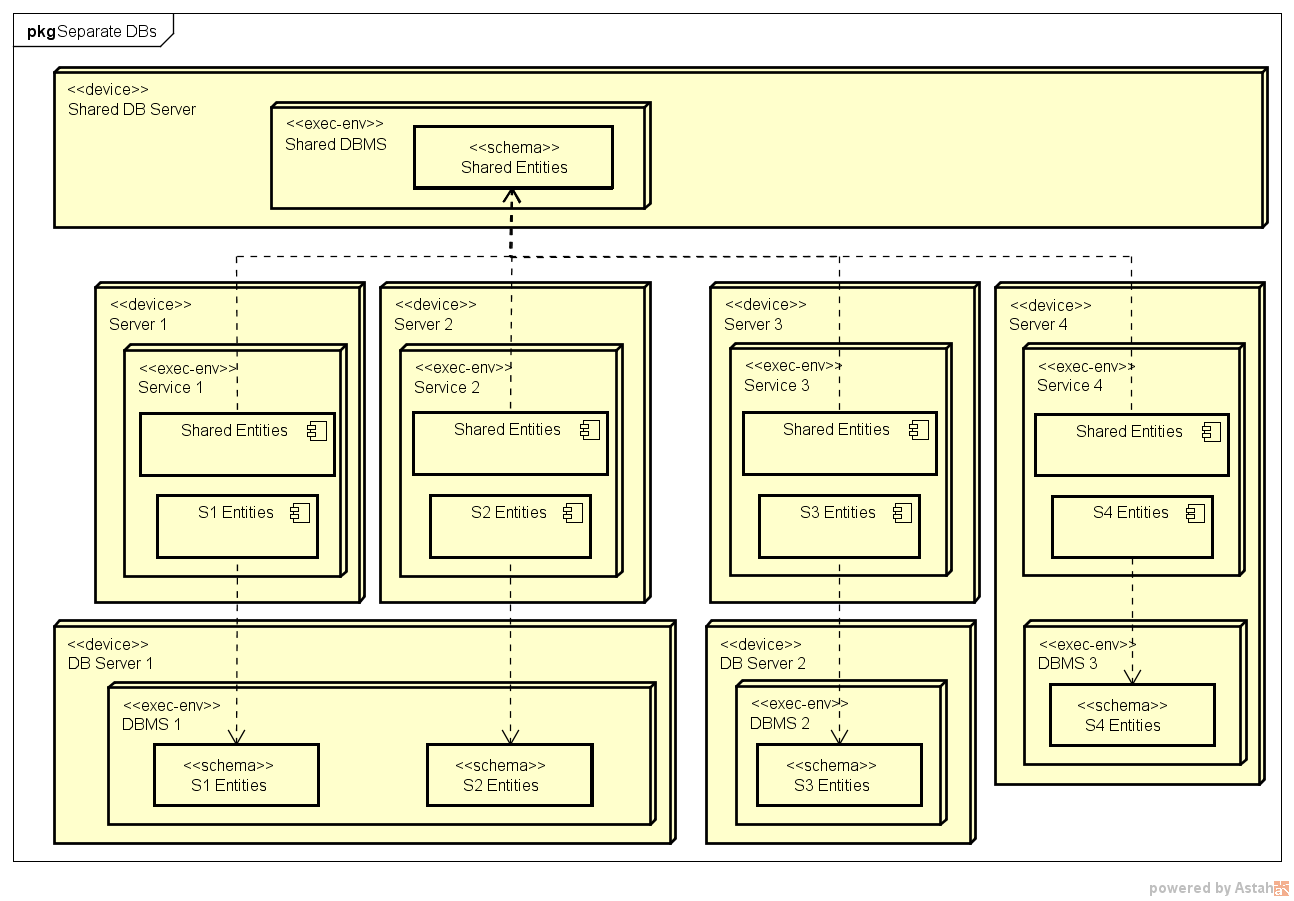
\includegraphics[trim=39 42 18 48,clip,width=0.92\paperwidth]{diagrams/separate-dbs.png}
%    \end{adjustwidth}
%    \caption{Separate databases example.}
%    \label{fig:separate-dbs}
%\end{figure}

In figure \ref{fig:separate-dbs}, there is a shared database that contains the entity data that is shared across services.
Service 1 and 2 are deployed on separate servers but share a single database server that hosts different tables for each service.
Service 3 has communicates with its own database server that hosts its tables.
Service 4 uses a database that is running on the same server as the service.

Each of these approaches have their own advantages and disadvantages.
A key consideration is whether a service has enough unique data to make it worth creating a separate database for just the service.
If most data is shared between services, it may be easier to implement the system with just a single shared database.
If there is some data that is unique to some services, a single database server
with either logical partitioning of the data or even indepedent database services,
may provide enough performance for the system.
A separate database server for some or all services provides greater flexibility for scaling,
if database performance is likely to become a bottleneck for the service.
Running an independent database on the same server as the service provides easier communication with the database
and may suit cases where an independent database is useful but it is not large enough to warrant to run on its own server.


\section{Conclusion}

Service-based architecture is an approach to designing a distributed system that is not too complex.
Domain services provide natural modularity and deployability characteristics in the architecture design.
Well designed service APIs improve the encapsulation and hide implementation details of the services.
